%%%Template designed by Adam Glesser September 9, 2008
%%%All rights reserved (and deserved) 
%%%The only thing you should mess with on this line is the word problems.
%%%If this is a problem set, leave it as problems.
%%%If this is a solution set, change it to solutions.
\documentclass[12pt,solutions]{article}

%%%Here you should replace my name with your name
\newcommand{\prof}{Katie Henry \\ David Snyder \\ Adi Renduchintala}
%%%Make this your course number than leave it alone
\newcommand{\subj}{}
%%%Change the number 1 to which problem set you're on
\newcommand{\psnumber}{} %This is the Problem Set #
%%%Change the due date as needed
\newcommand{\duedate}{\date}  
%%%Change the topic as needed
\newcommand{\topic}{MLCD Project}


%%%%%%%%%%%%%%%You don't need to mess with anything in this section%%%%%%%%
\newif\ifisproblemset
\PassOptionsToClass{11pt,12pt}{article}
\DeclareOption{problems}{\isproblemsettrue}
\DeclareOption{solutions}{\isproblemsetfalse}
\ExecuteOptions{solutions}
\ProcessOptions\relax


\usepackage{amsmath, amssymb}
\usepackage{amsfonts}
\usepackage{multicol,parskip}
\usepackage{graphicx,booktabs}
\usepackage{tikz}
\usetikzlibrary{bayesnet}
\setlength{\oddsidemargin}{0pt} \setlength{\evensidemargin}{0pt}
\setlength{\textwidth}{6.5in} \setlength{\topmargin}{-.5in}
\setlength{\textheight}{8.5in}

\newlength{\toppush}
\setlength{\toppush}{2\headheight} \addtolength{\toppush}{\headsep}

%%%This command makes the title. Don't mess with it, unless you want to change the name Problem Set
%%%or Solution to Problem Set to something else.
\newcommand{\htitle} 
{
    \noindent\vspace*{-\toppush}\newline\parbox{6.5in}
    {
        \vspace{-.85cm}
        \prof\hfill \ 
	 \today
	\vspace*{-.5ex}\newline
        \mbox{}\hrulefill\mbox{}
    }
    \vspace*{1ex}\mbox{}\newline
    \begin{center}{
        \large\bf{Progress Report} }\end{center}
}

%%%This command makes the headers. Don't mess with it.
\newcommand{\handout}
{
    \thispagestyle{empty}
    \markboth{\topic}{\topic}
    \pagestyle{myheadings}
    \htitle
}



%%%%%%%%%%%%%%%%%%%%%%%%%%%%%%%%%%%%%%%%%%%%%%%%%%%%%%%%%%%%%%%%%%%%


%%%%%%%%%%%%This next section contains custom macros%%%%%%%%%%%%%%%%%%
%If these don't fit your course, remove them and add your own


%This first one allows you to write limits faster. It takes 4 inputs:
%The variable, what it's approaching, if relevant which side and the function.
%For example, if you wanted to write the limit as a x goes to 3 from the left 
%side of the function x^2 + 3, you would write $\limit{x}{3}{-}{x^2+3}$. If 
%you didn't care about which side you would leave the third set of braces empty, i.e.,
%$\limit{x}{3}{}{x^2+3}$.
\newcommand{\limit}[3]{\lim\limits_{#1 \rightarrow #2}\ #3}

  
%This is a slightly faster way of writing derivatives. It takes 2 inputs:
%The first is the function your differentiating, the second is the variable 
%with respect to which you're differentiating. For example, if you want to
%write the the derivative of y with respect to x, you would type $\d{y}{x}$.
\renewcommand{\d}[2]{\dfrac{\mathrm{d}#1}{\mathrm{d}#2}}  

%This last macro creates a multicolumn list environment where the first input is the number of columns.
%Use this command when you plan on having so many parts to a problem, with each being very short to state
%that you would like to put the problems in several columns. An example of the syntax would be 
%\multilist{3}{
%\item first item
%...
%\item last item
%}
%This will create a list that displays in 3 columns. The 3 can be replaced by any natural number, but 2 and 3
%are the only one numbers likely to give readable output.
\newcommand{\multilist}[2] 
    {
        \begin{multicols}{#1}
            \begin{enumerate}
                #2
            \end{enumerate}
        \end{multicols}
    }
%%%For solutions sets:
%%%After you write the problem, the next line should be
%%%\solution{Type your solution in here}
\newcommand{\solution}{ 
  \medskip
  {\bf Solution:}
}     

\newcommand{\argmax}{\operatornamewithlimits{argmax}}
\newcommand{\argmin}{\operatornamewithlimits{argmin}}
\newcommand{\half}{\frac{1}{2}}
\newcommand{\dx}{\frac{\delta}{\delta x}}
\newcommand{\ab}{\mathbf{a}}
\newcommand{\X}{\mathbf{X}}
\newcommand{\Y}{\mathbf{Y}}
\newcommand{\bA}{\mathbf{A}}
\newcommand{\bmu}{\boldsymbol{\mu}}
\newcommand{\x}{\mathbf{x}}
\newcommand{\Xs}{\tilde{\mathbf{X}}}
\newcommand{\xs}{\tilde{\mathbf{x}}}
\newcommand{\y}{\mathbf{y}}
\newcommand{\sx}{\bar{\x}}
\newcommand{\tb}{\mathbf{t}}
\newcommand{\SG}{\mathbf{\Sigma}}
\newcommand{\ts}{\theta^*}
\newcommand{\tbi}{t_{b_i}}
\newcommand{\ptb}{\hat{t}_b}
\newcommand{\tv}{t_v}
\newcommand{\tvi}{t_{v_i}}
\newcommand{\ptv}{\hat{t}_v}
\newcommand{\ps}{\hat{s}}
\newcommand{\yh}{\hat{y}}
\newcommand{\M}{\mathbf{M}}
\newcommand{\R}{\mathbb{R}}
\newcommand{\D}{\mathbb{D}}
\newcommand{\I}{\mathbb{I}}
\newcommand{\N}{\mathbb{N}}
\newcommand{\E}{\mathbb{E}}
\newcommand{\T}{\mathbf{T}}
\renewcommand{\S}{\mathcal{S}}
\renewcommand{\th}{t_0}
\renewcommand{\v}{\mathbf{v}}
\newcommand{\w}{\mathbf{w}}
\newcommand{\W}{\mathbf{W}}
\newcommand{\p}{\mathbf{p}}
\newcommand{\wh}{\hat{\mathbf{w}}}
\newcommand{\wht}{\hat{\mathbf{w}}^T}
\newcommand{\whs}{\hat{\tilde{\mathbf{w}}}}
\newcommand{\whst}{\hat{\tilde{\mathbf{w}}}^T}
\newcommand{\ws}{\mathbf{w}^*}
\newcommand{\wst}{\mathbf{w}^{*T}}
\newcommand{\at}{\mathbf{a}^{T}}
\newcommand{\hth}{\hat{\theta}}
\newcommand{\bphi}{\boldsymbol{\phi}}
\newcommand{\btheta}{\boldsymbol{\theta}}
\newcommand{\dbphi}{\Delta\bphi}
\newcommand{\C}{\mathbf{C}}
\newcommand{\gd}{\nabla}
\newcommand{\hs}{\nabla^2}
\newcommand{\Cb}{\bar{C}}
\renewcommand{\labelenumi}{\arabic{enumi})}
\renewcommand{\labelenumii}{\alph{enumii})}
\providecommand{\norm}[1]{\lVert#1\rVert}

\newcommand{\solutionline}{
\begin{center}
\line(1,0){400}
\end{center}
}
    
%%%%%%%%%%%%%%%%%%%%%%%%%%%%%%%%%%%%%%%%%%%%%%%%%%%%%%%%%%%%%%%%%%%%%%%%%%%%%%%%%%%%
%%%%%%%%%%%%%%%%%%%%%%%%%%%%%%%%%%%%%%%%%%%%%%%%%%%%%%%%%%%%%%%%%%%%%%%%%%%%%%%%%%%%
%%%%%%%%%%%%%%%%%%%%%%%%%%%%%%%%%%%%%%%%%%%%%%%%%%%%%%%%%%%%%%%%%%%%%%%%%%%%%%%%%%%%
%%%%%%%%%%%%%%%%%%%%%%This is where the document begins%%%%%%%%%%%%%%%%%%%%%%%%%%%%%
%%%%%%%%%%%%%%%%%%%%%%%%%%%%%%%%%%%%%%%%%%%%%%%%%%%%%%%%%%%%%%%%%%%%%%%%%%%%%%%%%%%%
%%%%%%%%%%%%%%%%%%%%%%%%%%%%%%%%%%%%%%%%%%%%%%%%%%%%%%%%%%%%%%%%%%%%%%%%%%%%%%%%%%%%
%%%%%%%%%%%%%%%%%%%%%%%%%%%%%%%%%%%%%%%%%%%%%%%%%%%%%%%%%%%%%%%%%%%%%%%%%%%%%%%%%%%%
  
\begin{document}


%%%%%This stuff puts in the header and changes some spacing%%%%%%
\handout

\setlength{\parindent}{0pt}

The overall goal of this project is to develop a method for early detection of septic shock using continuous physiological data. We divide the problem into three parts: use topic modeling to learn features from the physiological data, derive a decision policy to decide what if any state the system should predict, and use a neural network to estimate the posterior probabilities for each state.

%%%%%%%%%%%%%%%%%%%%%%%%%%%%%%%%%%%%%%%%%%%%%%%%%%%%%%%%%%
%%%%%%%%%%Here is where the actual math begins%%%%%%%%%%%%
%%%%%%%%%%%%%%%%%%%%%%%%%%%%%%%%%%%%%%%%%%%%%%%%%%%%%%%%%%
\setcounter{section}{0}
\section{Feature Discovery}
\subsection{Problem Definition}
The goal of this section is to detect hidden states over the time-series data for each patient, that would augment features being used by subsequent prediction systems. A natural model for such a system is the HMM. Using these hidden state sequences as input tokens of a document, we intend to run Topic models over all the patient records to see if there is any groups of states or any patten in state sequences that either explain or help predict the onset of septic shock.
\subsection{Related Works}
As noted in our proposal, the prognosis of septic shock in critically ill patients has a lot of variability. There is no single monolithic notion of septic shock \cite{Shavdia2007} . There are several methods to approach feature discovery in time series data of this nature. \cite{Esbroeck2012hrt}  applied symbolic aggregate approximation SAX \cite{Lin2003sax} on physiological time series data. More recently, Time series topic models have also been developed, \cite{SariaThesis2011} these work directly on continuous time domain signals and extract latent motifs. In our approach, we would like to investigate an HMM based approach, to allow a hidden state to emit a vector observation for a single time instance, where each element in the observation vector represents the observation of each channel of data (ECG, blood pressure, oxygen saturation etc).
\subsection{Contribution}
The dataset contains patient heart rate data at a frequency of 2 Hz. Each sample has been obtained by computing statistics over a 2 minute window from a the original heart rate data. Thus, every 120th sample represents statistics from a non-overlapping region from the original data. The first task is to extract these samples per patient record. We intend to find hidden states that best explain this lower resolution data. Each state of our HMM model will cover a wider time window, our current estimate for length of observation window per state is 30 minutes.\\
We also intend to extend the HMM to a coupled HMM where the second set of observations would represent blood pressure, temperature or oxygen saturation. Ideally the second set of observations would be in close time sync with the Heart rate data. This would be a factor in deciding which data stream (temperature, blood pressure or oxygen saturation) we would use for the second observation layer in the coupled HMM. Another factor would be the availability of these streams for all patient records. \\
\subsection{Learning Problem}
We propose to learn a HMM and then extend it to a coupled HMM. The 2 layers of observation are heart rate and blood pressure, temperature or oxygen saturation.  We intent to learn the states sequence that would best explain the patient records. Below is a representation of this coupled HMM, with each variable defined.\\
\begin{figure}[ht]
  \begin{center}
    \begin{tabular}{cc}
      % model_reclas

\begin{tikzpicture}

% define nodes

% decisions



\node[latent, minimum size=9mm] (z0) {$z_{t-1}$};
\node[latent, right=2 cm of z0, minimum size=9mm] (z1) {$z_{t}$};
\node[latent, right =2cm of z1, minimum size=9mm] (z2) {$z_{t+1}$};

\node[obs, above=2cm of z0, minimum size=9mm] (o3) {$o^2_{t-1}$};
\node[obs, right=2 cm of o3, minimum size=9mm] (o4) {$o^2_{t}$};
\node[obs, right =2cm of o4, minimum size=9mm] (o5) {$o^2_{t+1}$};

\node[latent, below=2cm of z0, minimum size=9mm] (y0) {$y_{t-1}$};
\node[latent, right=2 cm of y0, minimum size=9mm] (y1) {$y_{t}$};
\node[latent, right =2cm of y1, minimum size=9mm] (y2) {$y_{t+1}$};

\node[obs, below=2cm of y0, minimum size=9mm] (o0) {$o^1_{t-1}$};
\node[obs, right=2 cm of o0, minimum size=9mm] (o1) {$o^1_{t}$};
\node[obs, right =2cm of o1, minimum size=9mm] (o2) {$o^1_{t+1}$};





% edges

\edge {z0,y0} {z1};
\edge {z0,y0} {y1};
\edge {z1,y1} {z2};
\edge {z1,y1} {y2};

\edge {z0} {o3};
\edge {z1} {o4};
\edge {z2} {o5};

\edge {y0} {o0};
\edge {y1} {o1};
\edge {y2} {o2};

\end{tikzpicture}
    \end{tabular}
  \end{center}
  \caption{Coupled HMM model}
\label{fig:coupled_hmm_fig}
\end{figure}
\begin{align*}
O^1 &= o^1_{0}, \ldots,o^1_{T},   \text{sequence of heart rate observations (statistics from a 30 min time window)}\\
O^2 &=o^2_{0}, \ldots,o^2_{T},  \text{sequence of blood pressure or oxygen saturation}\\
Z &=  z_{0}, \ldots,z_{T}, \text{sequence of ${O^2}$ related states}\\
Y &=  y_{0}, \ldots,y_{T},  \text{sequence of ${O^1}$ related states}\\
\end{align*}
\subsubsection{State Priors}
Using appropriate priors and initial values for states is crucial to restrain the system from straying away from what might be explanatory data. We intend to encode some of our prior intuitions in this model in the following manner. Let ${Y}$ represent the states for heart rate observations over the patient record. We have the following insights from the data that we would like to encode.\\
1. Bootstrap from Patient Records: Each patient record has a time stamp representing the presence of SIRS, Sepsis, Severe Sepsis or Septic Shock. While this time stamps are not exact (that is, they are marked when the clinician happens to observe the symptoms and there is no guarantee that it was the precise moment of onset) we can still get statistics from the time region surrounding the clinicians observation of the symptoms. Using this technique we can get good initial guesses for statistics (such as means, and variances i.e. modeling the observation as a Guassian) for 4 states. It might also be preferable to model the observation given the state as a Beta distribution as we know that Heart rate can never be negative (which a gaussian in theory will allow).\\
2. Low Heart Rate Variability: Apart from the 4 states with we intend to bootstrap our model with states that have priors to restrict their parameters. One of the key insights regarding the onset of septic shock is reduction in heart rate variability. This informs us that one of the statistics that we need to compute from each 30 min time window should be a good indication of variability. Thus, simply getting mean heart rate for a 30 min duration would not be a good statistic. We intend to initialize a "Low Variability" state to capture this trend.
3. High Heart Rate Variability: The opposite state from the pervious would be the "High Variability" state where the 30 min window shows significant variation.\\
4. Reduction in Variability State: This state would be initialized such that there is variability across the earlier samples which slowly decline as we reach the end of the time window. One way to achive this is to place a prior over the slope of a statistic such as change in variable from beginning of window to the end. A negative slope indicates reduction of variability.\\
Similar set of priors and initialization methods can be applied to the states corresponding to the ${Z}$ chain as well. It's important to note that some experimentation would be required to get a sense of these priors, they should be restrictive enough to coerce the model in the general direction we want, but also allow for discovery of states, and states sequences. We do not have plans for priors over state transitions.



\section{Reliable Classification}

\subsection{Problem Definition}
\begin{figure}[ht]
  \begin{center}
    \begin{tabular}{cc}
      % model_reclas

\begin{tikzpicture}

% define nodes

% decisions

\node[latent,minimum size=9mm] (up) {$u_{t-1}$};
\node[const, left=2cm of up,minimum size=9mm] (ud) {$\ldots$};
\node[latent, right=3cm of up,minimum size=9mm] (ut) {$u_{t}$};
\node[latent, right=3cm of ut,minimum size=9mm] (un) {$u_{t+1}$};
\node[const, right=2cm of un,minimum size=9mm] (uf) {$\ldots$};
% truth
\node[const, above=2cmof up,xshift=-3cm,minimum size=9mm] (yd) {$\ldots$};
\node[latent, above=2cm  of up,minimum size=9mm] (yp) {$y_{t-1}$};
\node[latent, right=3cm  of yp, minimum size=9mm] (yt) {$y_{t}$};
\node[latent, right=3cm  of yt,minimum size=9mm] (yn) {$y_{t+1}$};
% prediction
\node[latent, above=of yp, xshift=-1cm,minimum size=9mm] (yhp) {$\hat{y}_{t-1}$};
\node[latent, above=of yt, xshift=-1cm,minimum size=9mm] (yht) {$\hat{y}_{t  }$};
\node[latent, above=of yn, xshift=-1cm,minimum size=9mm] (yhn) {$\hat{y}_{t+1}$};
\node[const, right=3cm  of yhn,minimum size=9mm] (yf) {$\ldots$};
% observation
\node[obs, above=of yhp,minimum size=9mm] (xp) {$x_{t-1}$};
\node[obs, above=of yht,minimum size=9mm] (xt) {$x_{t}$};
\node[obs, above=of yhn,minimum size=9mm] (xn) {$x_{t+1}$};
% intervention
\node[obs, right=1cm of xp,minimum size=9mm] (rp) {$r_{t-1}$};
\node[obs, right=1cm of xt,minimum size=9mm] (rt) {$r_{t}$};
\node[obs, right=1cm of xn,minimum size=9mm] (rn) {$r_{t+1}$};


% edges

\edge {xp,yd} {yhp};
\edge {xt,yp} {yht};
\edge {xn,yt} {yhn};

\edge{rp, yhp} {yp};
\edge{rt, yht} {yt};
\edge{rn, yhn} {yn};
\edge {yn} {yf};
\edge {yp, ud} {up};
\edge {yt, up} {ut};
\edge {yn, ut} {un};
\edge {un} {uf};

% plates

\plate {} {(yp)(yt)(yn)(up)(ut)(un)}{};

\end{tikzpicture}
    \end{tabular}
  \end{center}
  \caption{Reliable Classifier model as a Bayesian network}
\label{fig:reclas_bnet}
\end{figure}


\begin{align*}
X &= x_0, x_1, \ldots, x_T \text{ sequence of observations}\\
R &= r_0, r_1 \ldots, r_T \text{ sequence of clinical interventions}\\
\hat{Y} &= \yh_0, \yh_1, \ldots, \yh_T \text{ sequence of predicted class labels, $\yh_i \in \{1,\ldots, C\}$}\\
Y&=y_0,y_1,\ldots,y_T \text{ sequence of true labels, $y_i \in \{1,\ldots, C\}$}\\
U&=u_0,u_1,\ldots,u_T \text{ a decision policy, $u_i \in \{1,\ldots, C, C+1\}$}\\
S &\in \R^{C+1 \times C \times T}, S_{i,j}^{(t)} \text{ is the cost of choosing label $i$ instead of label $j$ at time $t$}\\
\bar{C} &= \{1,\ldots, C\} \text{ set of possible classes}\\
\hat{C} &= \{1,\ldots, C,C+1\} \text{ set of possible decisions}
\end{align*}

Our goal is to learn a decision policy that allows us to make the optimal decision at time $T$ given a sequence of observations and a user-defined cost function.

At each time $t$ the system either chooses the class $c \in \{1,\ldots, C\}$ that minimizes the expected loss over the time sequence $0\ldots T$ or it refuses to make a decision, corresponding to choosing $c = C+1$. Each $\yh_t$ is a probability distribution over possible the possible classes $\bar{C}$. If there is a clinical intervention $r_t$ at the current time $t$, e.g.\ a doctor prescribes pressors or performs some other action that provides a diagnosis, we define $P(y_t=j)$ to be $P(y_t=j|r_t)$. However, since we are performing a continuous monitoring task, the majority of time points will not have a clinical intervention associated with it. In these cases we use the distribution from the classifier $\yh_t$ and define $P(y_t=j)$ to be $P(\yh_t=j|x_t, y_{t-1})$. We then feed the distribution $y_t$ to our classifier so that the predicted distribution over classes $\yh_{t+1}$ incorporates knowledge about clinical interventions into the classification process. Instead of defining the distribution $y_t$ as either $r_t$ or $\yh_t$, we could instead define it as a mixture of the two distributions based on our confidence in the classifier's predictions. 

The decision $u_t$ is influenced by the distribution over all possible class labels $y_t$ and the previous decision $u_{t-1}$. The motivation for allowing the previous decision to influence the current decision is two-fold. First this can act as a smoothing function and capture the intuition that patients show a gradual transition from one disease state to the next, and prevents situations like repeatedly alternating between two disease states instead of staying in one state until the classifier is sufficiently confident to advance to a new disease state. The second benefit of this dependency between successive decisions is that it allows us to prevent overly long rejection periods, where the classifier continuously refuses to predict. We can do this by progressively down-weighting the probability of rejection given the history of rejection.

\subsection{Related Work}

By adding the notion of rejection (i.e.\  refusing to predict), the classifier is able to avoid misclassification, by instead refusing to predict. As stated by Chow \cite{Chow1970} the optimal strategy is one that minimizes the rate of rejection. For a single time point, Chow shows how to formulate the decision policy of when to reject in terms of a rejection threshold. He similarly formulates the error in terms of that same threshold by noting that the expected cost of error is the expected cost of rejecting minus the expectation of being correct. This rejection threshold can then relate the expected cost of rejecting to the expected cost of misclassification and allow the user to trade off between them. 

Grall-Ma\"{e}s and  Beauseroy \cite{GrallMaes2009} extend the optimal decision framework by allowing an observation to be assigned to a subset of the classes. Assigning an observation to the set of all classes corresponds to refusing to predict and assigning an observation to a set with only one class corresponds to predicting that class without ambiguity. Grall-Ma\"{e}s and  Beauseroy derive the optimal decision policy for assigning an observation to a set given a cost matrix and performance constraints. Performance constraints are, for example, the false positives for this class must be below a given threshold or the false positives for a given subset must be below this level.

Santaniello et al.\ \cite{Santaniello2012} formulate a transition detection problem where they learn a decision policy to decide when a change of state has occurred in a time sequence. In particular, they derive a decision policy for quickest detection, where they want to detect the change point as early as possible with sufficient confidence. To encourage early detection, they include the expected distance of the current time from the actual change time in the cost function. 


\subsection{Contribution}
For the task of sepsis prediction and continuous patient monitoring in general, we want to derive a generic optimal decision policy for time series data where we allow the system to refuse to predict. Moreover, we allow for a user-defined cost function that can be asymmetric, e.g.\ assigning different costs for false positives or negatives for different classes, and that can change over time. This task is different than transition detection in that we do not assume there is only one transition point and we do not assume that the subject even has to transition.


\subsection{Simulation}

In order to test the reliable classification, we generate synthetic data from four overlapping Gaussians, where each Gaussian corresponds to a different class.

We use Kevin Murphy's BayesNet and CRF Matlab toolkits to implement a model to compute $\hat{Y}$ for the synthetic data. We then use these marginal probabilities at each time step to implement the learning problem as described below. For the simulation we do address the situation where we have a doctor intervention (i.e.\ $R=\emptyset$). 

We will consider how different parameterizations of the cost matrix allow us to trade off between the cost of misclassification and the cost of refusing to predict. We will also investigate how to set the cost matrix to encourage early detection.

\subsection{Learning Problem}
Our goal is to learn a decision policy that allows us to minimize the expected loss over the entire time sequence of observations.
The expected posterior loss at time $t$ of making decision $u_t=i$ given that the true label is $y_t=j$ and the previous decision was $u_{t-1}=h$ as follows:

\begin{align}
\E[L(u_t|y_t, u_{t-1})] &= \min_{u_t} \Big\{ \sum_{i \in \hat{C}} \sum_{j \in \bar{C}} S_{i,j}^{(t)} P(y_t=j)P(u_t=i|u_{t-1})\I(u_t=i)\Big\}\\
&= \min_{u_t \in \hat{C}} \Big\{ \sum_{j \in \bar{C}} S_{u_t,j}^{(t)} P(y_t=j)P(u_t|u_{t-1})\Big\}
\label{eqn:exploss}
\end{align}

We use dynamic programming to learn the optimal decision policy over the time sequence, with a discounting factor $\beta \in [0,1]$ to adjust the importance of past observations.

Let $V(y_T)$ be the value of the expected posterior loss minimized by a decision policy $\{u_t\}_{t=0}^{T}$. At time $T$ we make the decision $u_T$ that is the argmin of (\ref{eqn:bellman}).

\begin{align}
V(y_T) &= \min_{\{u_t\}_{t=0}^{T}} \Big\{ \sum_{t=0}^T \beta^{T-t}\E[L(u_t|y_t, u_{t-1})] \Big\}\\
&= \min_{u_T \in \hat{C}} \Big\{  \beta^{0}\E[L(u_T|y_T, u_{T-1})] + \min_{\{u_t\}_{t=0}^{T-1}} \beta \sum_{t=0}^{T-1} \beta^{T-1-t}\E[L(u_t|y_t, u_{t-1})] \Big\}\\
&= \min_{u_T \in \hat{C}} \Big\{  \E[L(u_T|y_T, u_{T-1})] + \beta V(y_{T-1})\Big\} \label{eqn:bellman}
\end{align}

From this we see that the system will either make the decision $u_T = c \in \bar{C}$ that minimizes the expected loss over the sequence or it will refuse to predict, equivalent to choosing $u_T = C+1$. 

Computing the expected loss with dynamic programming, where we maintain a vector of the class costs from the previous time step, requires $C(C+1)+4$ operations at each time point, so the overall complexity is $O(TC^2)$. For space efficiency, it is only necessary to maintain the cost vector from the previous time step.


\section{Neural Networks for Posterior Estimation}

\subsection{Problem Definition}
The goal of this section is to train Deep Neural Networks (DNN) to estimate the probability of developing a disease state given a sequence of
physiological data. Here, the task is early prediction of septic shock in ICU patients with a documented infection. Heart rate is used as input to
the DNN. We will estimate the probability of an ICU patient developing a form of sepsis $P(sepsis \mid S)$ where $S$ is window into the 
heart rate timeseries. DNNs have produced state of the art performance in a number of domains. The paradigm gains efficacy over traditional neural networks in part due to its ability to extract multiple layers of features during its unsupervised pretraining. Onset of sespsis is believed to be preceded by reduced complexity of the cardiac waveform, one such highlevel predictor of the disease we speculate that the neural network may learn. 

\subsection{Related Work}

At present, deep learning the task of sepsis prediction appears relatively unexplored. However, these techniques have been successfully applied to classification and prediction on other physiological time series. \cite{wulsin2011modeling} applied Deep Belief Networks (DBNs), a related technique to the task of anomaly detection in clinical EEG records. The group found that 
DBNs produced comparable results to other state of art methods, but significantly faster. They found
that using the raw EEG waveform showed improved performance in an
anomaly detection task over engineered features.
These results underscore the advantage of deep learning methods in 
automatically uncovering useful features. \\

To obtain adequate performance a body of techniques and tricks need to be considered. In \cite{hinton2012deep} speech recognition groups at Google, Microsoft, IBM and University of Toronto share various techniques for improving DNN performance. For instance, one should consider techniques for
preventing overfitting by certain restrictions on weight updating and smart initialization of weights.

\subsection{Approach and Learning Problem}

Equation (6) describes
the output of a neuron $j$ given the weighted commulative input $x_j$ (7). 
\begin{align}
y_{j} = \frac{1}{1+e^{-x_{j}}} \\
x_{j} = b_{j} + \sum_{i}y_{i}w_{ij} \\
p(sepsis \mid S) = \frac{1}{1 + exp(x_{sepsis})}
\end{align}

Equation 8 presents the most simplistic task, the probability
of sepsis given some some sequence of physiological signals $S$. We can
extend this to multi-class classification by a generalization
of this output function, \textit{softmax}. Given the simple task, the 
target function is simply (9) where $t_{j}$ is the correct class label (eg, sepsis or not sepsis).
\begin{align}
J = -\sum_{j} t_{j} log(y_{j})
\end{align} \\

Typically DNNs are pretrained layerwise by treating each layer as a 
Restricted Boltzmann Machine (RBM), a technique which we will implement for this project. \\

Acquiring good performance with DNNs relies upon proper weight initialization, pretraining, topology and other considerations described in \cite{vesely2013sequence, hinton2012deep}. We will also compare the performance of the DNN using the raw heart rate data versus a derived dataset with standard features. 

\subsection{Data}

The data for this task consists of heart rate sampled at 2 Hz derived from the MIMIC II Waveform Database. For DNN training, we use a 486 record subset which 
serves as the training, dev, and test sets. 
Each record contains heart rate for an ICU patient with SIRS, severe sepsis or septic shock, with at least
12 hours preceding the event.

\bibliographystyle{plain}

\bibliography{PhysMod,dnn,ref}

\end{document}
